\maketitle

\section{Logic minimization}

A general optimization criteria for multi-level logic are to Minimize
some combination of:
\begin{enumerate}
\item Area occupied by the logic gates and interconnect;
\item the Critical Path Delay of the longest path through the logic;
\item the Degree of Testability of the circuit, measured in terms of the percentage
of faults covered by a specified set of test vectors, for an appropriate fault model
(Eg., single stuck faults, multiple stuck faults, etc.);
\item Power consumed by the logic gates.
\end{enumerate}

In this course, we will start with two-level multi-input circuits and a criteria
based on the number of gates/transistors/diodes.

\section{Programmable Logic Arrays}
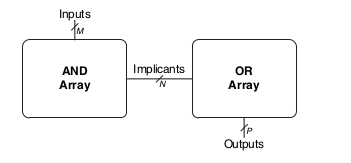
\includegraphics[width=0.5\linewidth]{figures/PLA-abstract.png}
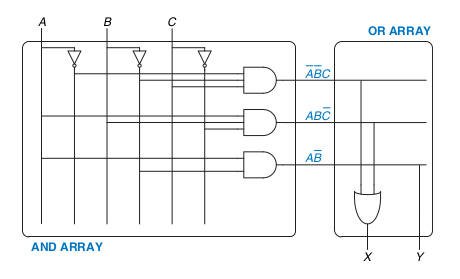
\includegraphics[width=0.5\linewidth]{figures/PLA-logic.png}

\section{Two-level circuits}
The cost that we are going to consider in this class depend upon:
\begin{enumerate}
\item Number of gates.
\item Number of input to the gates.
\end{enumerate}
More gates need more transistors, more area on the chip. More-inputs the gate
need more transistors within each gate. Number of gate inputs can be considered
secondary criterion to the number of gates.

\begin{example}
  Find the cost of the following Boolean expression $X = \bA\bB C + AB\bC + A\bB$.
\end{example}

\begin{prob}
  Find the cost of the following Boolean expression $X = A\bB C + \bA B\bC + \bB
  C$.
\end{prob}

\section{Terminology for K-maps}
Running Example: $f = \sum m(0, 1, 2, 3, 7) = \bx_1 + x_1 x_2 x_3$.
\begin{description}
  \item[Literal] A single variable or its complement. Example: $\bx, x_1, x_2, x_3$
  \item[Implicant] A product term which is true for a function. All minterms are
    implicants. Example: $x_1
    x_2 x_3$, $\bx_1$, $m_0 = \bx_1\bx_2\bx_3$, $\bx_1 x_3$, $\bx_1 \bx_3$.
  \item [Prime Implicant] An implicant that cannot be combined into fewer
    literals. Example: $\bx_1, x_2x_3$.
  \item [Essential Prime Implicant] An implicant that cannot be combined into
    fewer literals. Example: $x_2x_3$.
  \item [Cover] : List of Prime Implicants that account for all $f = 1$.
  \item [Cost]: Number of gates (excluding not gate on literals) and number of
      inputs to each gate.
\end{description}

\begin{example}
  Find minimum cost expression for the function $f(x_1, x_2, x_3) = \prod M(4, 5, 6)$
\end{example}
\vspace{10em}

\begin{prob}
  Find minimum cost expression for the function $f(x_1, x_2, x_3) = \prod M(2, 5, 6)$
\end{prob}
\vspace{10em}

\subsection{Incompletely specified functions or Don't cares}

\begin{figure}[h!]
  \centering
  \begin{circuitikz}
    \draw (0,0) node[seven segment val=0 dot off box on]{};
    \draw (1,0) node[seven segment val=1 dot off box on]{};
    \draw (2,0) node[seven segment val=2 dot off box on]{};
    \draw (3,0) node[seven segment val=3 dot off box on]{};
    \draw (4,0) node[seven segment val=4 dot off box on]{};
    \draw (5,0) node[seven segment val=5 dot off box on]{};
    \draw (6,0) node[seven segment val=6 dot off box on]{};
    \draw (7,0) node[seven segment val=7 dot off box on]{};
    \draw (8,0) node[seven segment val=8 dot off box on]{};
    \draw (9,0) node[seven segment val=9 dot off box on]{};
  \end{circuitikz}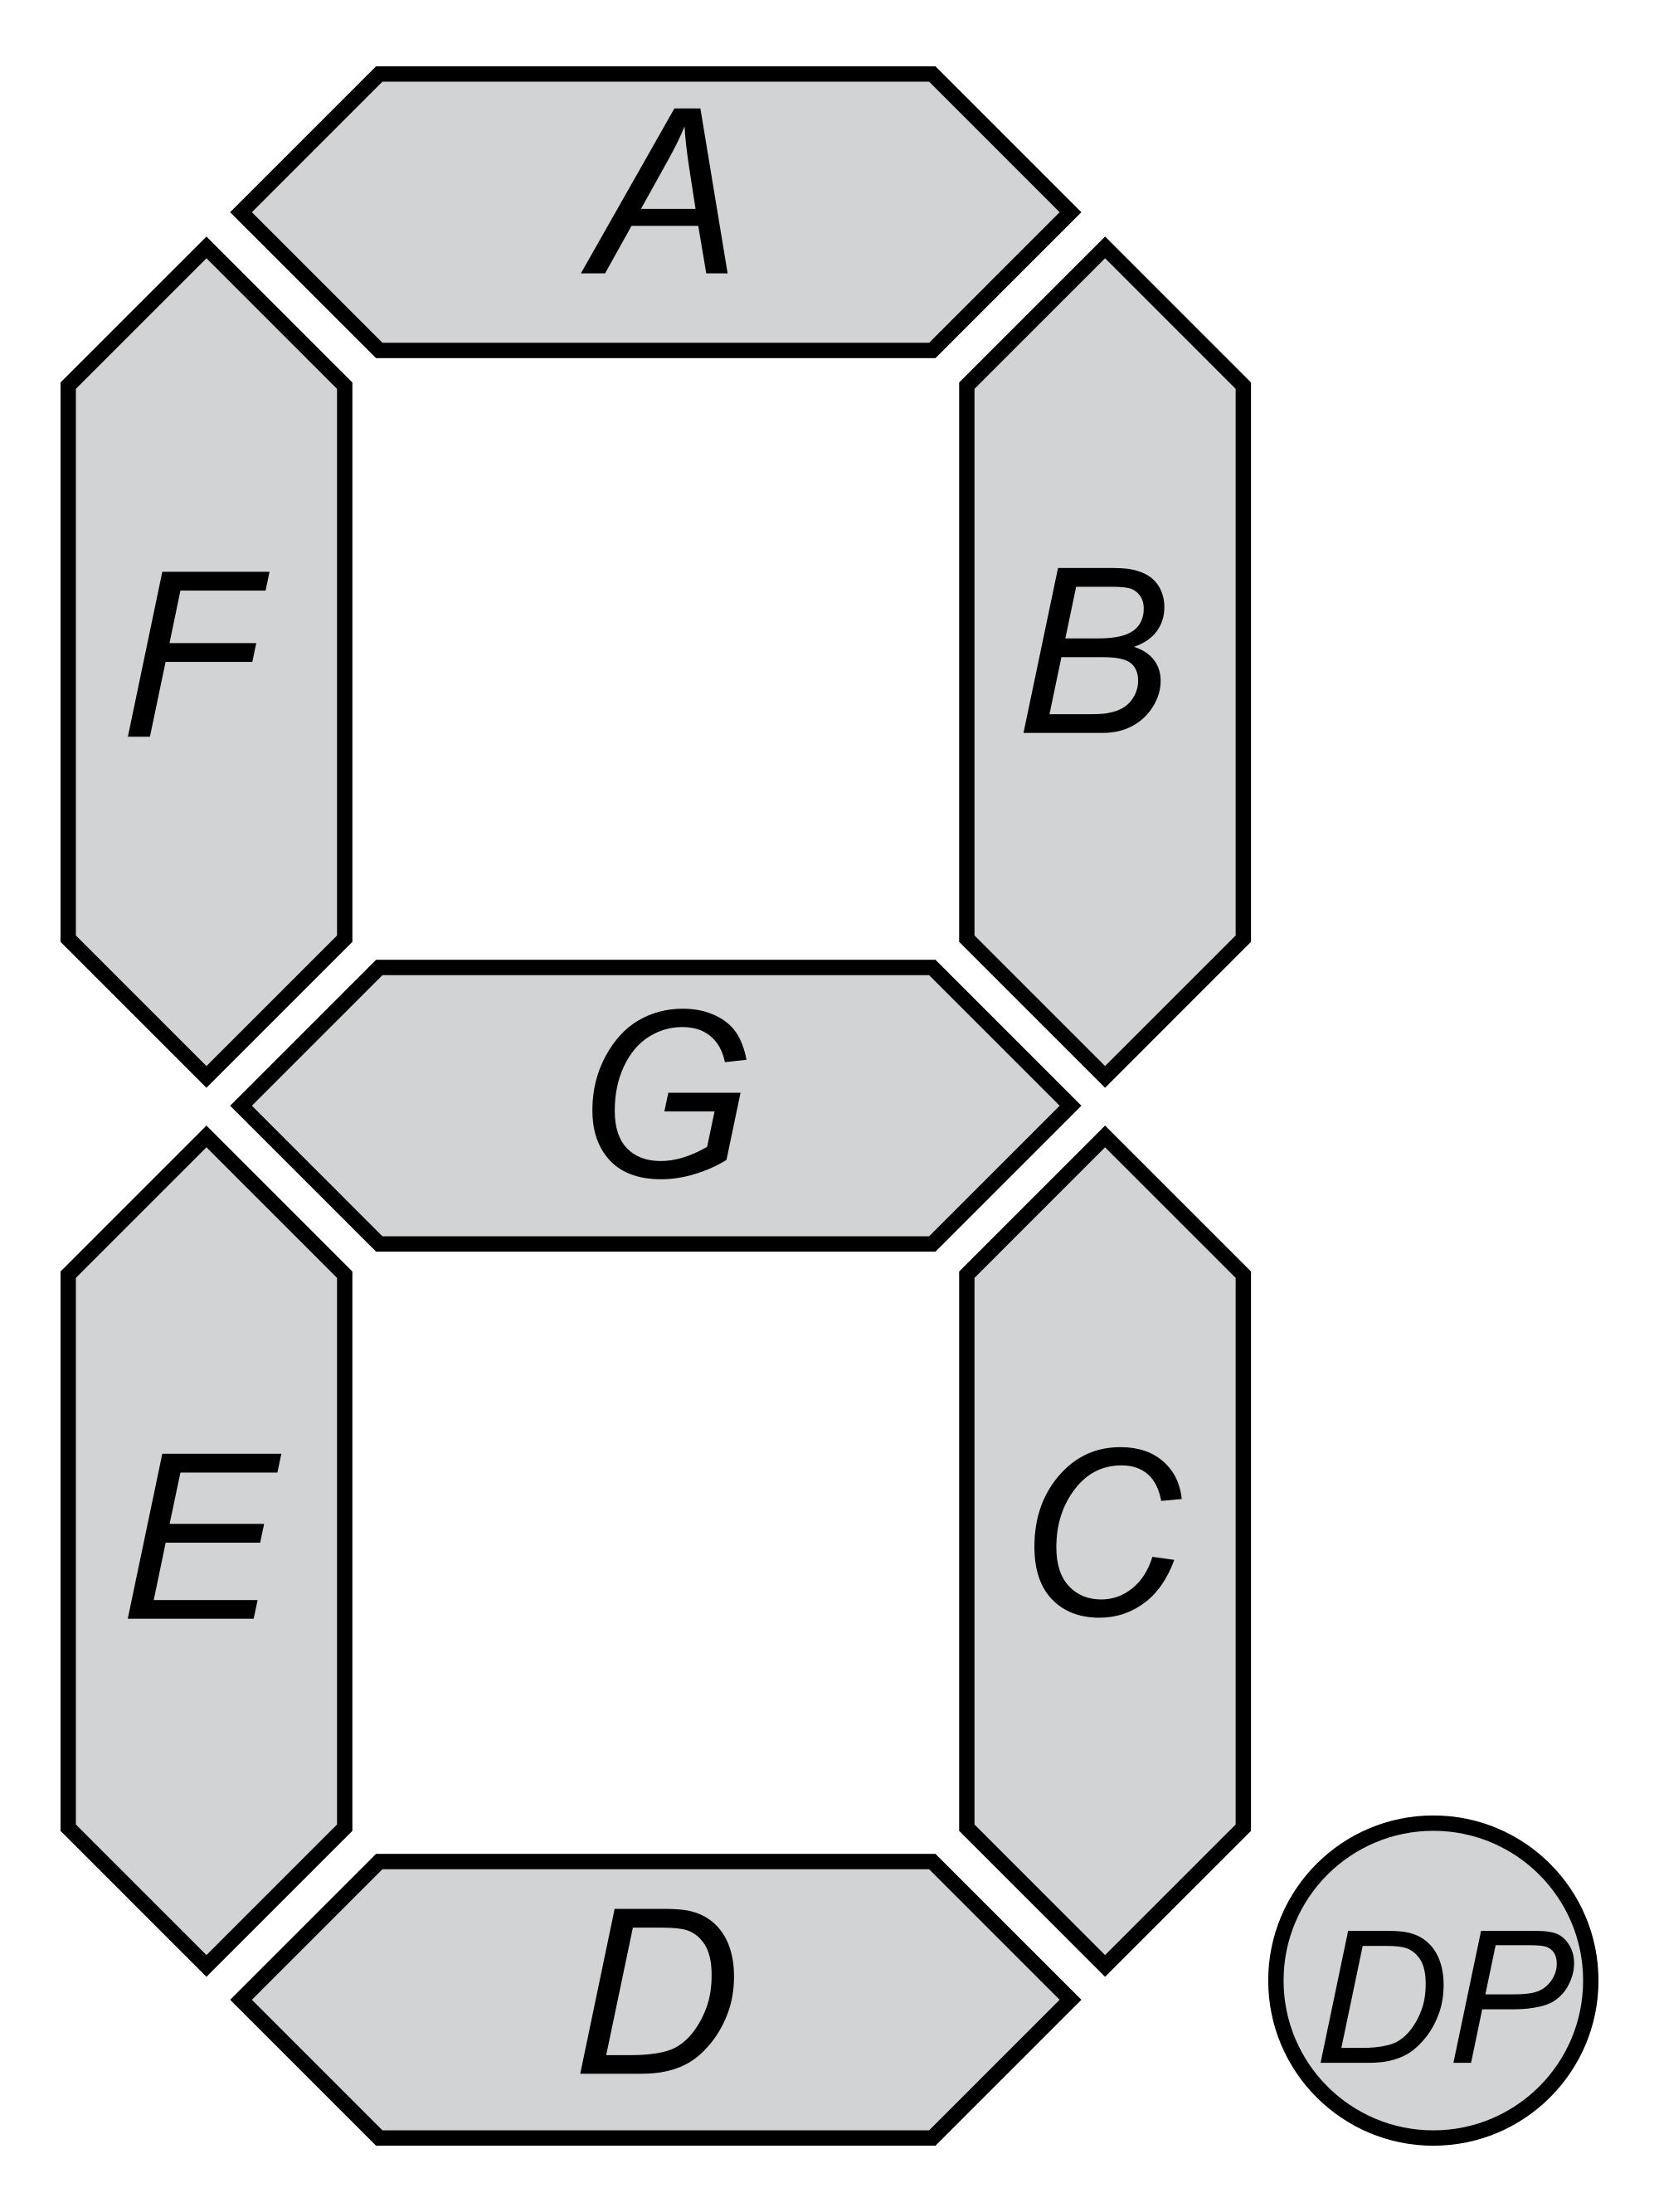
\includegraphics[width=0.1\linewidth]{figures/seven_segment.png}
  \caption{7 Segment Representations of Each Integer}
  \label{sevensegs}
\end{figure}

\begin{tabular}{cccc|c}
  \toprule
  \multicolumn{4}{c|}{BCD Value} & LED Segment \\
  $D_3$ & $D_2$ & $D_1$ & $D_0$ & E \\
  \midrule
  0 & 0 & 0 & 0 & 0\\
  0 & 0 & 0 & 1 & 1\\
  0 & 0 & 1 & 0 & 0\\
  0 & 0 & 1 & 1 & 1\\
  0 & 1 & 0 & 0 & 1\\
  0 & 1 & 0 & 1 & 1\\
  0 & 1 & 1 & 0 & 0\\
  0 & 1 & 1 & 1 & 1\\
  1 & 0 & 0 & 0 & 0\\
  1 & 0 & 0 & 1 & 1\\
  1 & 0 & 1 & 0 & d\\
  1 & 0 & 1 & 1 & d\\
  1 & 1 & 0 & 0 & d\\
  1 & 1 & 0 & 1 & d\\
  1 & 1 & 1 & 0 & d\\
  1 & 1 & 1 & 1 & d\\
  \bottomrule
\end{tabular}

\begin{example}
  Find minimum cost expression for the function
  \[ f(x_1, \dots, x_4) = \sum m(2, 4, 5, 6, 10) + D(12, 13, 14, 15) \]
\end{example}
\vspace{10em}

\begin{prob}
  Find minimum cost expression for the function
  \[ f(x_1, \dots, x_4) = \sum m(0, 2, 4, 6, 7, 8, 9, 13) + D(1, 12, 15) \]
\end{prob}
\vspace{10em}